\graphicspath{ {./YX/} }

\begin{solution}

  \subsection{Mathematical Formulation}
    The Couette Flow obeys the following equations of motion:
    \begin{align}
      \nabla\cdot\mathbf{u}&=0 \label{eq:continuity}\\
      \rho\left(\frac{\partial\mathbf{u}}{\partial t}+\mathbf{u}\cdot\nabla\mathbf{u}\right)
      &=-\nabla P+\mu\nabla^2\mathbf{u} \label{eq:momentum}
    \end{align}
    Eq.(\ref{eq:continuity}) is known as the equation of continuity, and Eq.(\ref{eq:momentum}) describes the conservation of momentum. Other assumptions in this problem are translated as follows:
    \begin{enumerate}
      \item Steady
        \begin{equation}
          \frac{\partial (\cdot)}{\partial t}=0
        \end{equation}
      \item Fully developed
        \begin{equation}
          \frac{\partial\mathbf{u}}{\partial x}=0
        \end{equation}
      \item Two-dimensional
        \begin{equation}
          \frac{\partial (\cdot)}{\partial z}=0
        \end{equation}
      \item Zero pressure-gradient
        \begin{equation}
          \nabla P=0
        \end{equation}
      \item No-slip boundary
        \begin{equation}
          \mathbf{u}\big|_{y=-h}=0, \quad
          \mathbf{u}\big|_{y=h}=U\hat{\mathbf e}_x
        \end{equation}
    \end{enumerate}
    Putting them all together, we have the well-posed problem for $\mathbf{u}=u(y)\hat{\mathbf{e}}_x+v(y)\hat{\mathbf{e}}_y$:
    \begin{align}
      \frac{\partial v}{\partial y}&=0 \\
      v\frac{\partial u}{\partial y}&=\frac{\mu}{\rho}\frac{\partial^2 u}{\partial y^2} \\
      v\big|_{y=-h}=0&,\quad v\big|_{y=h}=0 \\
      u\big|_{y=-h}=0&,\quad u\big|_{y=h}=U
    \end{align}

\end{solution}



\begin{solution}
    
  \subsection{The Velocity Field}
    We first note that $v$ has its own independent boundary problem, \emph{i.e.}
    \begin{align}
      \frac{\partial v}{\partial y}&=0 \\
      v\big|_{y=-h}=0&,\quad v\big|_{y=h}=0
    \end{align}
    whose solution is:
    \begin{align}
      v=0
    \end{align}
    Plugging it back, we rewrite the problem for $u$:
    \begin{align}
      \frac{\partial^2 u}{\partial y^2}&=0 \\
      u\big|_{y=-h}=0&,\quad u\big|_{y=h}=U
    \end{align}
    So the solution for $u$ is:
    \begin{align}
      u=\frac{U}{2}\left(1+\frac{y}{h}\right)
    \end{align}
    Putting them together we have the full solution for the velocity field:
    \begin{align}
      \mathbf{u}=\frac{U}{2}\left(1+\frac{y}{h}\right)\hat{\mathbf{e}}_x
    \end{align}
    \begin{figure}[H]
      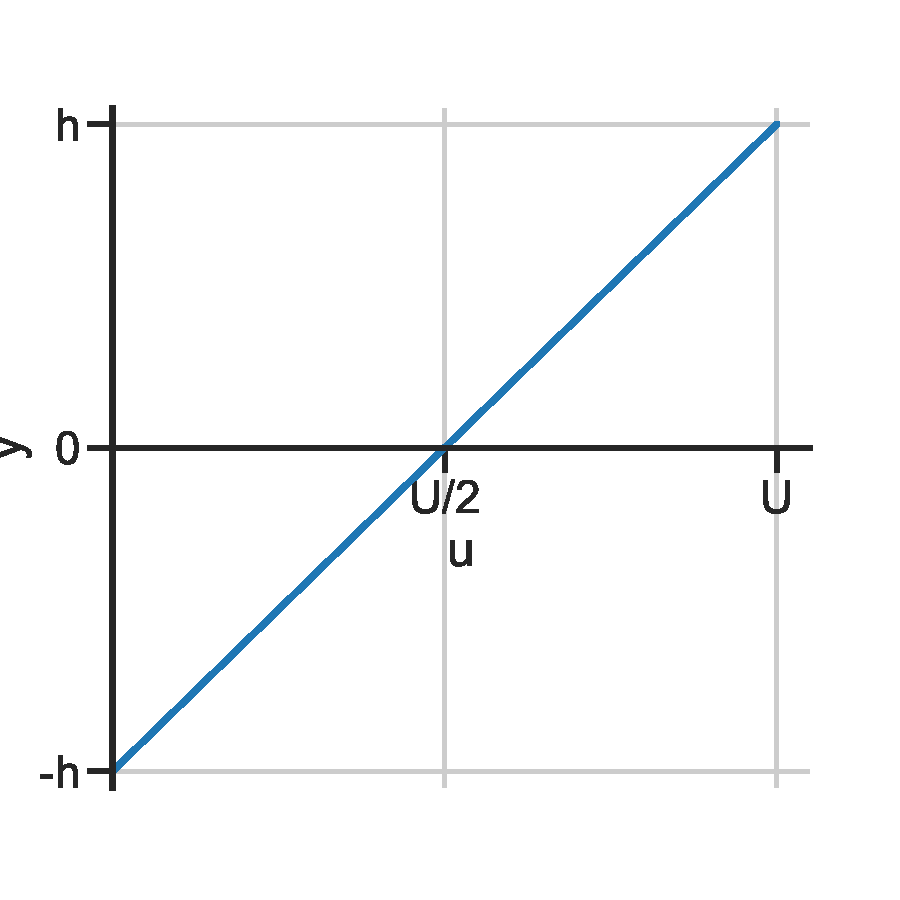
\includegraphics[scale=0.5]{YX/velocity_profile.pdf}
      \centering
      \caption{Velocity Profile}
    \end{figure}
    
\end{solution}



\begin{solution}

  \subsection{The Vorticity Field}
    \begin{align}
      \omega=\nabla\times\mathbf{u}=-\frac{U}{2h}\hat{\mathbf{e}}_z
    \end{align}
    
  \subsection{The Shear Stress}
    \begin{align}
      \tau=\mu\left(\nabla\mathbf{u}+\nabla\mathbf{u}^T\right)=\frac{\mu U}{2h}\left(\hat{\mathbf{e}}_{xy}+\hat{\mathbf{e}}_{yx}\right)
    \end{align}
  
  \subsection{The Volume Flow Rate}
    \begin{align}
      Q=\int_{-h}^{h}\!u~\text{d}y=Uh
    \end{align}

  \subsection{The Average and Maximum Velocity}
    \begin{align}
      u_{ave}&=\frac{Q}{2h}=\frac{U}{2} \\
      u_{max}&=U
    \end{align}
    

\end{solution}